%! Author = thibaultchausson
%! Date = 28/11/2022

%!TEX root = ../main.tex

\subsection{Création de l'ontologie en Python}

Pour ce faire, nous utiliserons le package \href{https://linuxfr.org/news/owlready-un-module-python-pour-manipuler-les-ontologies-owl}{owlready2} qui permet de créer des ontologies en Python.
Les données seront extraites de la base de données de WikiData, nous interrogerons cette base de données par l'API mis à disposition par la librairie \href{https://github.com/LeMyst/WikibaseIntegrator#execute-sparql-queries}{wikibaseintegrator}.

Dans les étapes précédentes nous avons récupéré le nom des animaux avec les différentes sous-classes qui leurs sont liées.
Nous nous sommes rapidement rendu compte que des classes sont en commun avec d'autres animaux.
Par exemple, nous avons un animal qui a pour sous-classe \og éléphant \fg{} et \og mammifère \fg{} un autre a pour sous-classe \og éléphant d'Asie \fg{} et \og éléphant \fg{}, donc nous devons créer une classe éléphant d'Asie qui découle d'éléphant qui elle-même découle de mammifère.


De plus, si nous devons ajouter des animaux nous pouvons être confronté au fait qu'un animal n'a pas de classe, donc nous créons une classe générique \textit{SansFamille}.

Pour générer l'ontologie mous suiverons ces étapes : 
\begin{enumerate}
    \item Création d'une IRI
    \item Création de la classe \textit{Animalia(Thing)}
    \item Création des sous-classes qui découlent de \textit{Animalia} et des sous-classes précédement créées
    \item Définition de la classe \textit{Image} avec son nom et si elle est reconnue ou non
    \item Définir les exclusions (la notion d'exclusion n'existe pas à proprement parlé dans owlready2)
    \item Définition des propriété : \textit{Contient}, \ldots\ et des \textit{CaracteristiqueMorphologique} avec par exemple, \textit{plume}, \ldots\
    \item Ajout des animaux
    \item Ajout des images liées à un animal et si oui ou non l'image est reconnue 
    \item Enregistrement de l'ontologie
\end{enumerate}

\subsection{Visualisation de l'ontologie avec Protégé}

Pour comprendre plus finement l'ontologie créée par Python nous utiliserons le logiciel Protégé\cite{protege} développé par Stanford.


\begin{figure}[!h]
    \begin{center}
        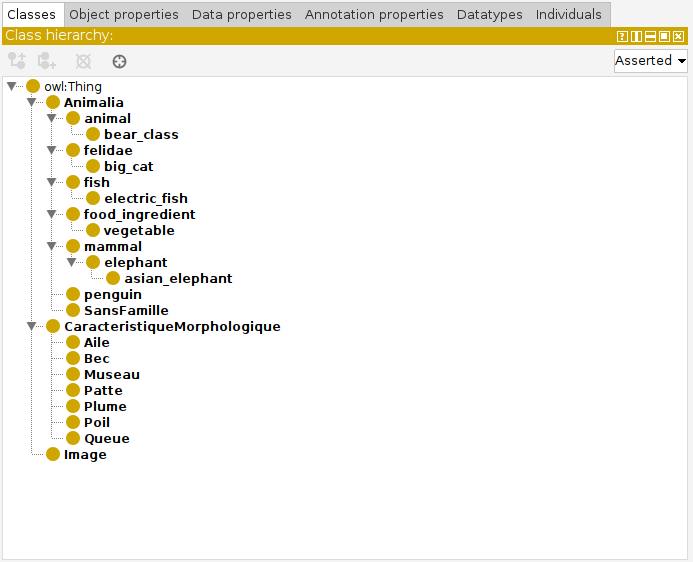
\includegraphics[scale=0.35]{./ressources/Classe.png}
        \caption{Classe de l'ontologie \label{fig:classe}}
    \end{center}
\end{figure}

Dans la figure \ref{fig:classe}, nous remarquons l'ensemble des classes créées par notre code source en fonction des informations récupérées sur WikiData, par exemple la classe \textit{big\_cat} hérite de \textit{fellidae}, qui hérite elle-même de \textit{Animalla}. 

De plus, nous remarquons que l'ensemble des classes sont en minuscule et sans espace, ceci pour simplifier la création de ces-dernières.


\begin{figure}[!h]
    \begin{center}
        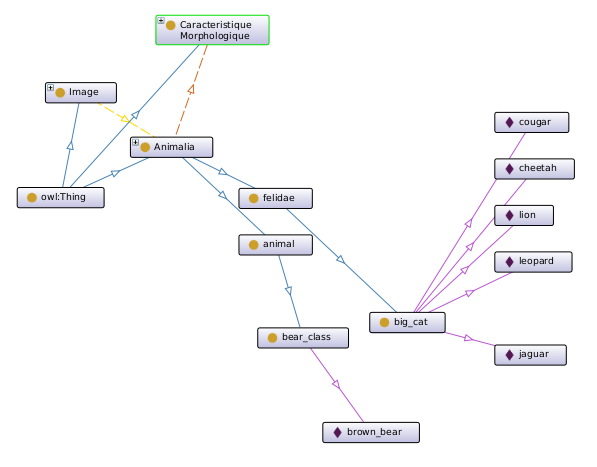
\includegraphics[scale=0.42]{./ressources/graphe2.png}
        \caption{Graphe de l'ontologie \label{fig:graphe}}
    \end{center}
\end{figure}

Sur la figure \ref{fig:graphe}, nous visualisons l'ensemble des liens issues des relations entre les animaux. 
Nous en déduisons que les cougars et les lions doivent se ressembler car ils font partie de la même classe.


\begin{paddingTab}
    \begin{customFrameXML}
    <big_cat rdf:about="#lion">
      <rdf:type rdf:resource="http://www.w3.org/2002/07/owl#NamedIndividual"/>
    </big_cat>
    \end{customFrameXML}
    \captionof{lstlisting}{Information d'un animal dans l'ontologie \label{cs:owlAnimal}}
\end{paddingTab}


\begin{figure}[!h]
    \begin{center}
        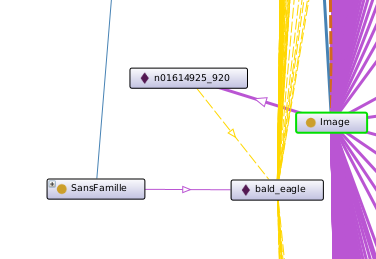
\includegraphics[scale=0.55]{./ressources/image.png}
        \caption{Image de l'ontologie \label{fig:image}}
    \end{center}
\end{figure}

Il nous à aussi été demandé de montrer la relation entre les images et les animaux, sur la figure \ref{fig:image}, il y a la classe \textit{image} qui contient \textit{n01614925\_920} qui est relié à \textit{bald\_eagle}, et ainsi nous savons que cette image est un Pygargue à tête blanche qui a été ou non reconnu par notre modèle.
De plus nous précisons divers information comme l'URL de l'image, son format, \ldots\

\begin{paddingTab}
    \begin{customFrameXML}
    <Image rdf:about="#n01443537_8719">
      <rdf:type rdf:resource="http://www.w3.org/2002/07/owl#NamedIndividual"/>
      <Contient rdf:resource="#goldfish"/>
      <Reconnue rdf:datatype="http://www.w3.org/2001/XMLSchema#boolean">false</Reconnue>
      <URL rdf:datatype="http://www.w3.org/2001/XMLSchema#string">./ILSVRC/Annotations/CLS-LOC/train/n01443537/n01443537_8719.xml</URL>
      <Width rdf:datatype="http://www.w3.org/2001/XMLSchema#string">500</Width>
      <Height rdf:datatype="http://www.w3.org/2001/XMLSchema#string">376</Height>
      <Depth rdf:datatype="http://www.w3.org/2001/XMLSchema#string">3</Depth>
    </Image>
    \end{customFrameXML}
    \captionof{lstlisting}{Information d'une image dans l'ontologie \label{cs:owlImage}}
\end{paddingTab}


